\documentclass[eng,oneside]{mgr}
\usepackage[polish]{babel}
\usepackage[utf8]{inputenc}
\usepackage{polski}
\usepackage[hidelinks]{hyperref}
\usepackage{graphicx} 
\usepackage{listings}
\usepackage{color}
\frenchspacing
\usepackage{indentfirst}
\usepackage{caption}

\definecolor{mygreen}{rgb}{0,0.6,0}
\definecolor{mygray}{rgb}{0.5,0.5,0.5}
\definecolor{mymauve}{rgb}{0.58,0,0.82}

\lstset{ %
	backgroundcolor=\color{white},   % choose the background color
	basicstyle=\footnotesize,        % size of fonts used for the code
	breaklines=true,                 % automatic line breaking only at whitespace
	frame=single,  
	commentstyle=\color{mygreen},    % comment style
	escapeinside={\%*}{*)},          % if you want to add LaTeX within your code
	keywordstyle=\color{blue},       % keyword style
	stringstyle=\color{mymauve},     % string literal style
}

\author{Marcin Mantke}
\title{System zarządzania inteligentnym domem z wykorzystaniem Raspberry Pi oraz technologii internetowych.}
\engtitle{Smart house management system using Raspberry Pi and Web technologies.}
\supervisor{dr inż. Marek Piasecki}
\field{Informatyka (INF)}
\specialisation{Inżynieria systemów informatycznych (INS)}
\date{2015}

\begin{document}
\maketitle
\tableofcontents
\chapter{Wstęp}
\section{Ogólny opis projektu}
\section{Cel projektu}
\section{Wymagania}
\section{Ograniczenia}



\section{Przegląd wybranych rozwiązań}
\subsection{Domoticz.com}
Od czasu popularyzacji rozwiązań pokroju Arduino i Raspberry Pi, hobbystyczne projekty inteligentnych domów są coraz częściej realizowane. Sprzyja temu fakt, że ceny podzespołów wymaganych do realizacji projektu są coraz niższe, a osoby zainteresowane mają coraz więcej literatury dostępnej w Internecie. Takimi właśnie hobbystami byli twórcy platformy \textit{Domoticz}. Jest to zagraniczny serwis udostępniający multiplatformowe rozwiązania dla inteligentnych domów. Jest on skierowany głównie do hobbystów. Jak można przeczytać na stronie domowej projektu (\url{http://www.domoticz.com/}), \textit{Domoticz} jest systemem automatyki domowej, który pozwala na monitorowanie i konfigurację urządzeń, takich jak: światła, przełączniki, różnego rodzaju sensory i mierniki, jak np temperatury, deszczu, wiatru, UV, prądu, gazu i wody.

Serwis ten udostępnia biblioteki umożliwiające podłączenie sensorów oraz oprogramowanie jednostki bazowej systemu (zwykle Raspberry Pi). Jako, że udostępniane są biblioteki, a nie tylko gotowe moduły sprzętowe, całość jest bardziej elastyczna. Oczywiście są tu ograniczenia, zarówno hardware'owe, jak i software'owe, lecz są one mniejsze niż w przypadku gotowych rozwiązań.

Samo oprogramowanie jest darmowe (Licencja GNU), ze strony producenta możliwy jest zakup urządzeń współpracujących z jego systemem, jednak możliwe jest również tworzenie sensorów we własnym zakresie, przy użyciu posiadanych podzespołów oraz udostępnionych bibliotek.
\subsection{Fibaro}                                                                                              
Rozwiązania oferowane przez firmę \textit{Fibaro} mają odmienną filozofię od firmy \textit{Domoticz}. Firma ta jest ukierunkowana na rozwiązania komercyjne. Oferuje ona systemy automatyki budynkowej, składające się z gotowych podzespołów, które trzeba jedynie zainstalować w budynku oraz skonfigurować.

System umożliwia dodawanie własnych scenariuszy działania. Ich definiowanie zbudowane jest na wzór programowania \textit{Scratch} (\url{https://scratch.mit.edu/})

System Fibaro opiera się na topologii sieci typu \textit{mesh}. Urządzenia łączą się ze sobą za pośrednictwem protokołu \textit{Z-wave}.
\begin{figure}[h]
\centering
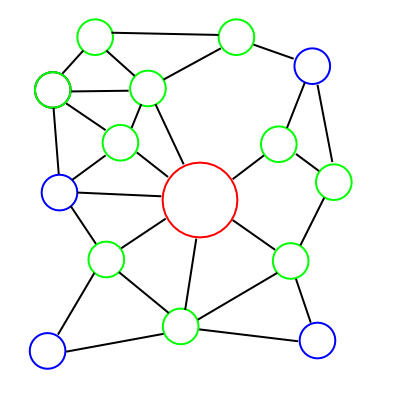
\includegraphics[width=0.7\linewidth]{mesh}
\caption{Schemat topoligii typu mesh.}
\label{fig:Mesh-Network}
\end{figure}

\section{Zarys koncepcji}
Koncepcyjnie, inteligentny dom można podzielić na 3 główne części. Są one od siebie ściśle zależne,
% Jednostka centralna
% Czujniki
% Aplikacja webowa
% Akcja - reakcja

\chapter{Architektura systemu}
\section{Topologia systemu}
\url{https://pl.wikipedia.org/wiki/Topologia_gwiazdy}
\chapter{Specyfikacja systemu}
\chapter{Wybrane technologie}
\section{Hardware}
\section{Software}
\subsection{Aplikacja internetowa}
Serwis internetowy wykonany został w oparciu o następujące technologie:
\begin{itemize}
	\item \textbf{Ruby on Rails} - wnętrze (back-end) portalu webowego, które odpowiedzialne jest za wykonywanie określonych zadań na podstawie danych otrzymanych z fasady (front-end),
	\item \textbf{AngularJS} - fasada (front-end) - jej zadaniem jest komunikacja z użytkownikiem (odbieranie od niego danych oraz przekazywanie ich do back-end'u). AngularJS jest frameworkiem JavaScript'owym, który wymaga stosowania wzorca projektowego \emph{MVC} (ang. Model-View-Controller).
\end{itemize}
Ponadto wykorzystane zostały następujące elementy:
\begin{itemize}
	\item \textbf{CoffeeScript} - język programowania kompilowany do JavaScriptu. Ponieważ CoffeeScript kompiluje się do JavaScriptu, programy mogą być krótsze o około $\frac{1}{3}$ bez strat dla szybkości działania,
	\item \textbf{Slim} – język oparty na szablonach (ang. template language), którego celem jest maksymalna redukcja składni HTML’owej poprzez usunięcie np. tagów zamykających. W efekcie otrzymujemy bardzo czytelny kod, oparty na wcięciach.
\end{itemize}

\subsection{Baza danych}
Jako system bazodanowy wykorzystany został MySQL w wersji 5.6. Niewątpliwymi zaletami tego systemu jest to, że posiada on wysoki stopień niezawodności, jest darmowy oraz powszechnie dostępny i wspierany.

\chapter{Implementacja}
\chapter{Testy}
\section{Aplikacja internetowa}
\subsection{Testy jednostkowe}
% Do testów jednostkowych dla aplikacji webowej użyliśmy biblioteki RSpec, służącej do testowania kodu Rubiego, ze wsparciem dla frameworka Rails. Wybraliśmy tą bibliotekę, ponieważ wspiera ona idee Model-View-Controller, w oparciu o którą powstała nasza aplikacja. Dużą wygodą jest również automatyczna konfiguracja środowiska testowego, która polega m. in.  na osobnej, testowej bazie danych, która jest tworzona na początku wykonywania testów i czyszczona po zakończeniu każdego przypadku testowege.

% RSpec posiada bardzo intuicyjną składnie, przyjazna użytkownikowi naszym zdaniem. Testy podzielone są na 3 poziomową strukturę, każdy poziom zaczyna się słowem kluczowym:
% \begin{enumerate}
% 	\item ,,describe'' – tu definiujemy jaką funkcje/klasę/moduł ma sprawdzać dany zbiór testów,
% 	\item ,,context'' – to miejsce służy do określenia warunków testu,
% 	\item ,,it'' – mówi nam jak powinien się zachować testowany moduł.
% \end{enumerate}

% Przykładowy pojedynczy przypadek testowy:

% \begin{lstlisting}[language=Ruby, caption={RSpec test jednostkowy.}]
% RSpec.describe TripsController, :controller do #
% Describe'POST #create' do
% context 'with valid attributes' do
% it 'creates the trip' do
% login_user
% post :create, trip: attributes_for(:trip_with_path), format: :json
% expect(Trip.count).to eq(1)
% end
% end
% end
% end
% \end{lstlisting}

% Powyższy test ma za zadanie sprawdzić czy dane wysłane w odpowiednim formacie zapytaniem http post, przekazane do funkcji ,,create'' klasy ,,TripsController'' stworzą w bazie danych nowy rekord w tabeli Trip. 

% Dla ułatwienia wprowadzania atrybutów do testowanych metod lub dodawania rekordów do bazy danych nie wykorzystując napisanych przez siebie metod posłużyliśmy się biblioteką ,,FactoryGirl'', która implementuje wzorzec projektowy fabryki. Definicja obiektu jest bardzo prosta:

% \begin{lstlisting}[language=Ruby, caption={Definicja FactoryGirl.}]
% FactoryGirl.define do 
% factory :full_trip, class: Trip do
% distance 100
% avg_rpm 2500
% avg_speed 94
% avg_fuel 8.9
% date '2015-05-14T21:23:11.510Z'
% mark 5.0
% user_id 1
% beginning 'Start'
% finish 'Finish'
% challenge_id nil
% engine_type_id 1
% engine_displacement_id 1
% end
% end
% \end{lstlisting}

% Poniżej znajduje się użycie metody "FactoryGirl.create'', która tworzy obiekt w bazie danych. Ten przykład ilustruje również strukturę zbioru testów dla pojedynczej metody:

% \begin{lstlisting}[language=Ruby, caption={Użycie FactoryGirl.}]
% describe 'GET #mytrips' do
% context 'with valid attributes' do
% let!(:login) { login_user }
% let(:current_user_id) { login.id }
% it 'renders all user\'s trips as json' do
% FactoryGirl.create(:engine_displacement)
% FactoryGirl.create(:engine_type)
% FactoryGirl.create(:fuel_consumption)
% FactoryGirl.create(:full_trip, user_id: current_user_id)
% get :mytrips, format: :json
% expect(response).to be_success
% json = JSON.parse(response.body)
% expect(json).not_to be_empty
% expect(json[0].length).to eq(20)
% end
% it 'renders empty array when user has no trips' do
% get :mytrips, format: :json
% expect(response).to be_success
% json = JSON.parse(response.body)
% expect(json).to be_empty
% end
% end

% context 'with user not logged in' do
% it 'redirects to login page' do
% FactoryGirl.create(:engine_displacement)
% FactoryGirl.create(:engine_type)
% FactoryGirl.create(:full_trip)
% get :mytrips, format: :json
% expect(response).to have_http_status(401)
% end
% end
% end
% \end{lstlisting}

% Stworzyliśmy 19 testów jednostkowych. Badaliśmy pokrycie kodu aplikacji testami narzędziem Rcov. Tą analizę uruchamialiśmy po każdym commicie do repozytorium, dlatego wiemy jak się to kształtowało od moment skonfigurowania Rcov w Jenkinsie:
% \begin{figure}[h]
% 	\centering
% 	%\includegraphics[width=0.8\linewidth]{}
% 	\caption{Wykres pokrycia kodu.}
% 	\label{fig:testy}
% \end{figure}

% Ostatecznie pokrycie kodu źródłowego testami jednostkowymi wynosi około 75\%. Rcov pokazuje również dokładnie, które linie kodu są testowane:
% \begin{figure}[h]
% 	\centering
% 	%\includegraphics[width=0.9\linewidth]{}
% 	\caption{Raport Rcov dla pliku trips\_controller.rb.}
% 	\label{fig:raport}
% \end{figure}
\chapter{Podsumowanie}

\begin{thebibliography}{inteligencja}
	\addcontentsline{toc}{chapter}{Bibliografia}

	\bibitem{inteligentne domy}
	Z. Piątek, \emph{Od automatyki budynkowej do inteligentnych domów}, dostępne pod adresem \url{http://automatykab2b.pl/}, aktualne na dzień 31.10.2015r.
	
	\bibitem{rails guide}
	\emph{Ruby on Rails Guides}, dostępne pod adresem: \url{http://guides.rubyonrails.org/},\\ aktualne na dzień 14.06.2015r.
	
	\bibitem{angular guide}
	\emph{AngularJS Developer Guide}, dostępne pod adresem: \url{https://docs.angularjs.org/guide}, aktualne na dzień 14.06.2015r.
	
\end{thebibliography}
\end{document}